\section{Écrans produits}
Plusieurs écrans exploitables ont été réalisés avec la nouvelle machine et l'ancienne machine pour les expositions suivantes au spray :
\begin{itemize}
    \item 5 secondes (ancienne machine + mesure manuelles)
    \item 10 secondes (ancienne machine + mesure manuelles)
    \item 15 secondes (nouvelle machine + mesure auto)
    \item 30 secondes (nouvelle machine + mesure auto)
    \item 60 secondes (nouvelle machine + mesure auto)
\end{itemize}
Par exploitables on entend qu'ils ressemblent visuellement au résultat attendu décrit dans la \autoref{sec:fab_ecran_sit_init}.
\begin{figure}[H]
    \centering
    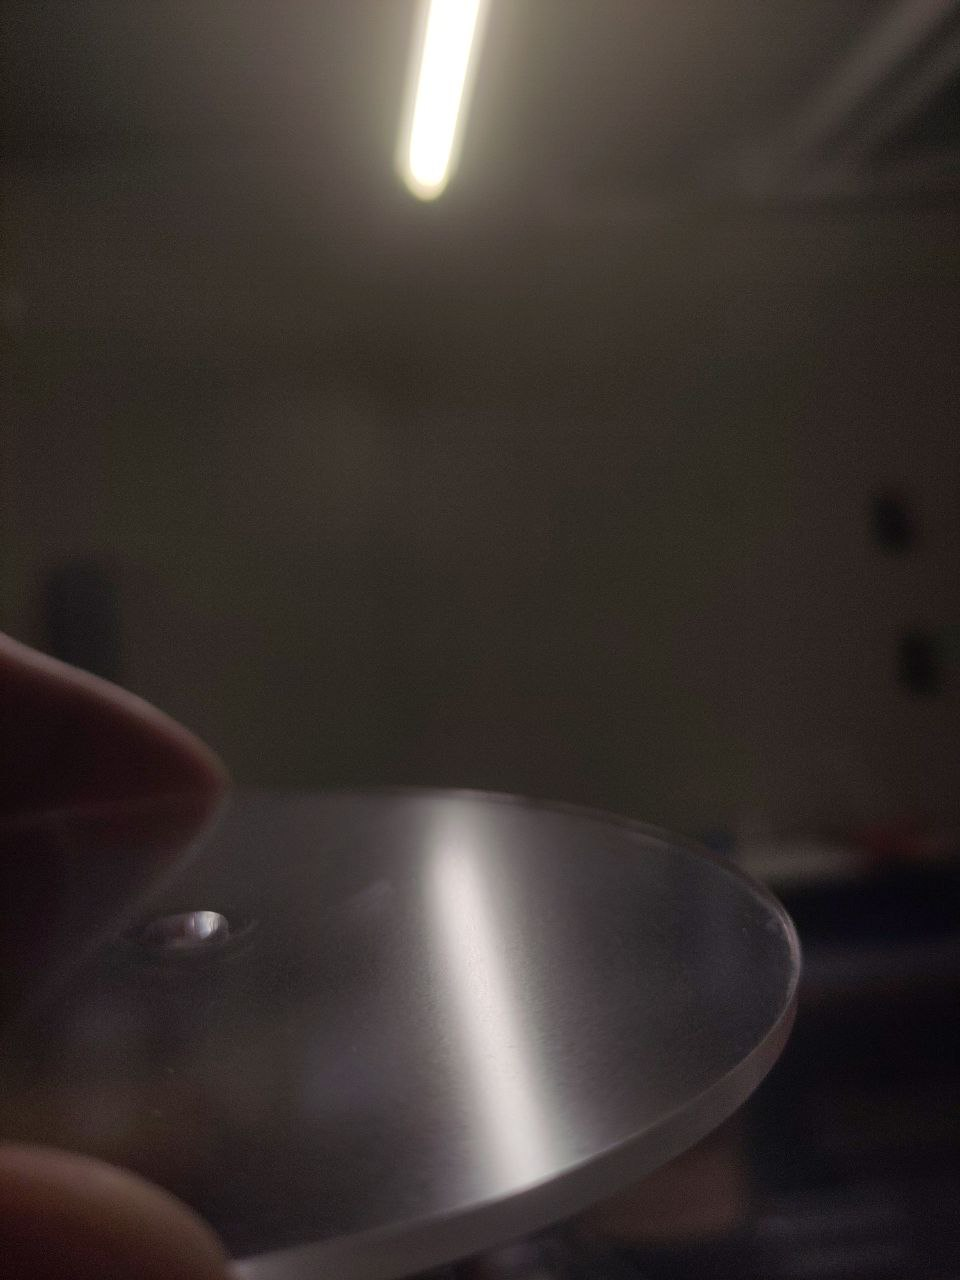
\includegraphics[width = 0.5\textwidth]{assets/figures/mesures/15_sec.jpeg}
    \caption{Écran 15 secondes}
\end{figure}

\begin{figure}[H]
    \centering
    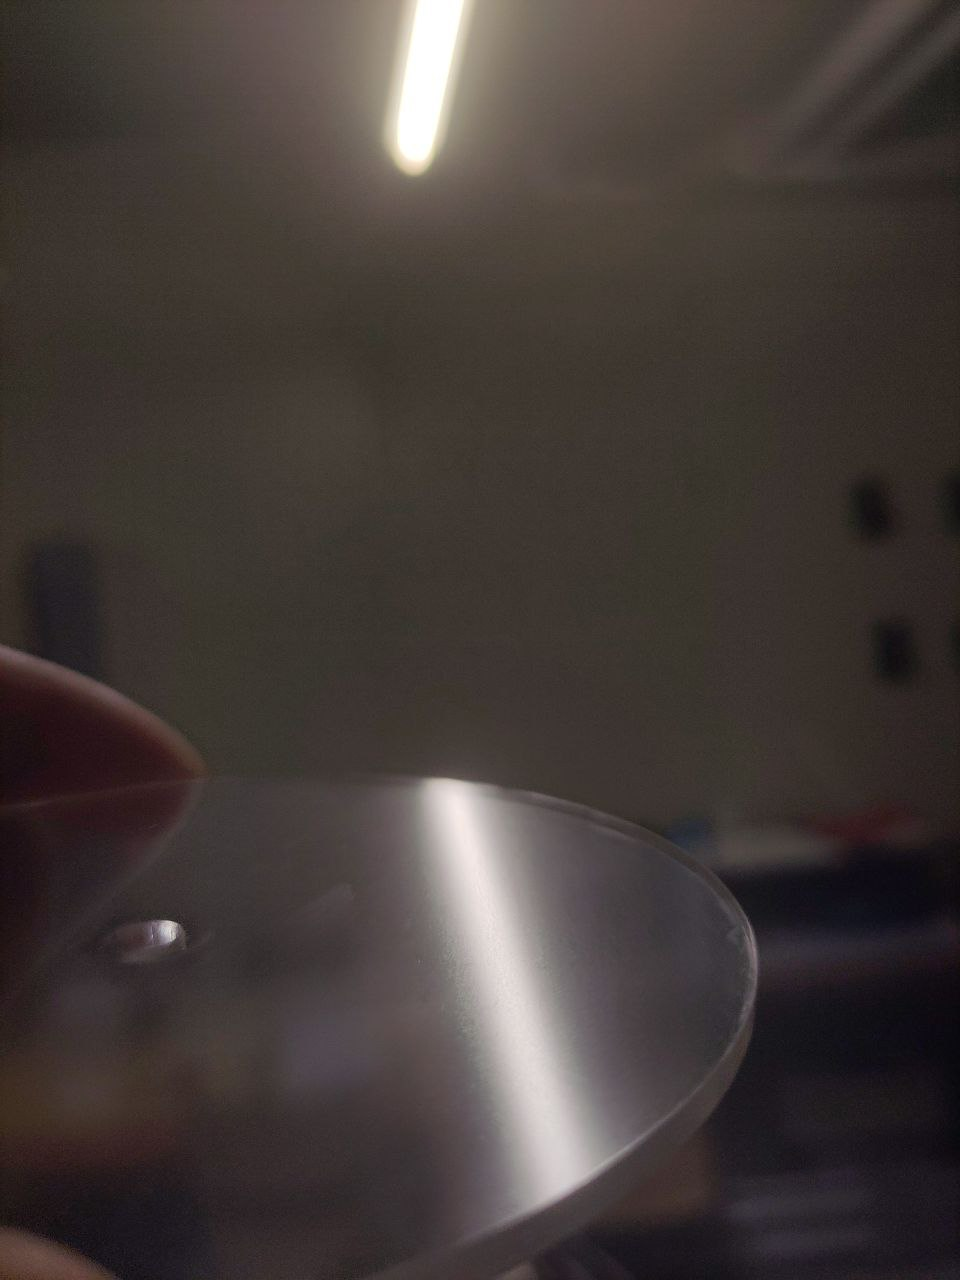
\includegraphics[width = 0.5\textwidth]{assets/figures/mesures/30_sec.jpeg}
    \caption{Écran 30 secondes}
\end{figure}

\begin{figure}[H]
    \centering
    \begin{subfigure}{.5\textwidth}
        \centering
        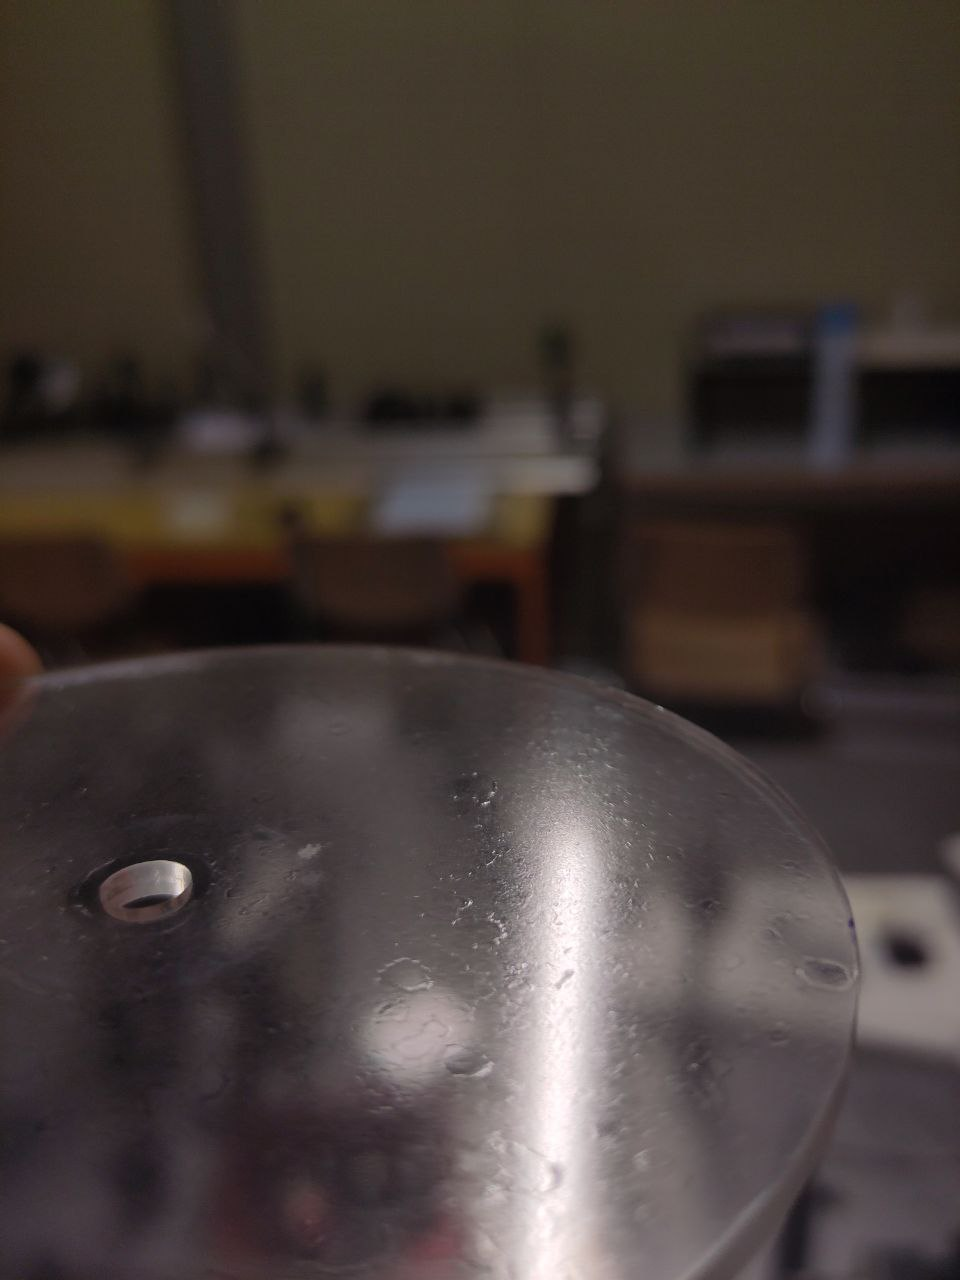
\includegraphics[width=1\linewidth]{assets/figures/mesures/60_sec.jpeg}
        \caption{Écran 60 secondes}
    \end{subfigure}%
    \begin{subfigure}{.5\textwidth}
        \centering
        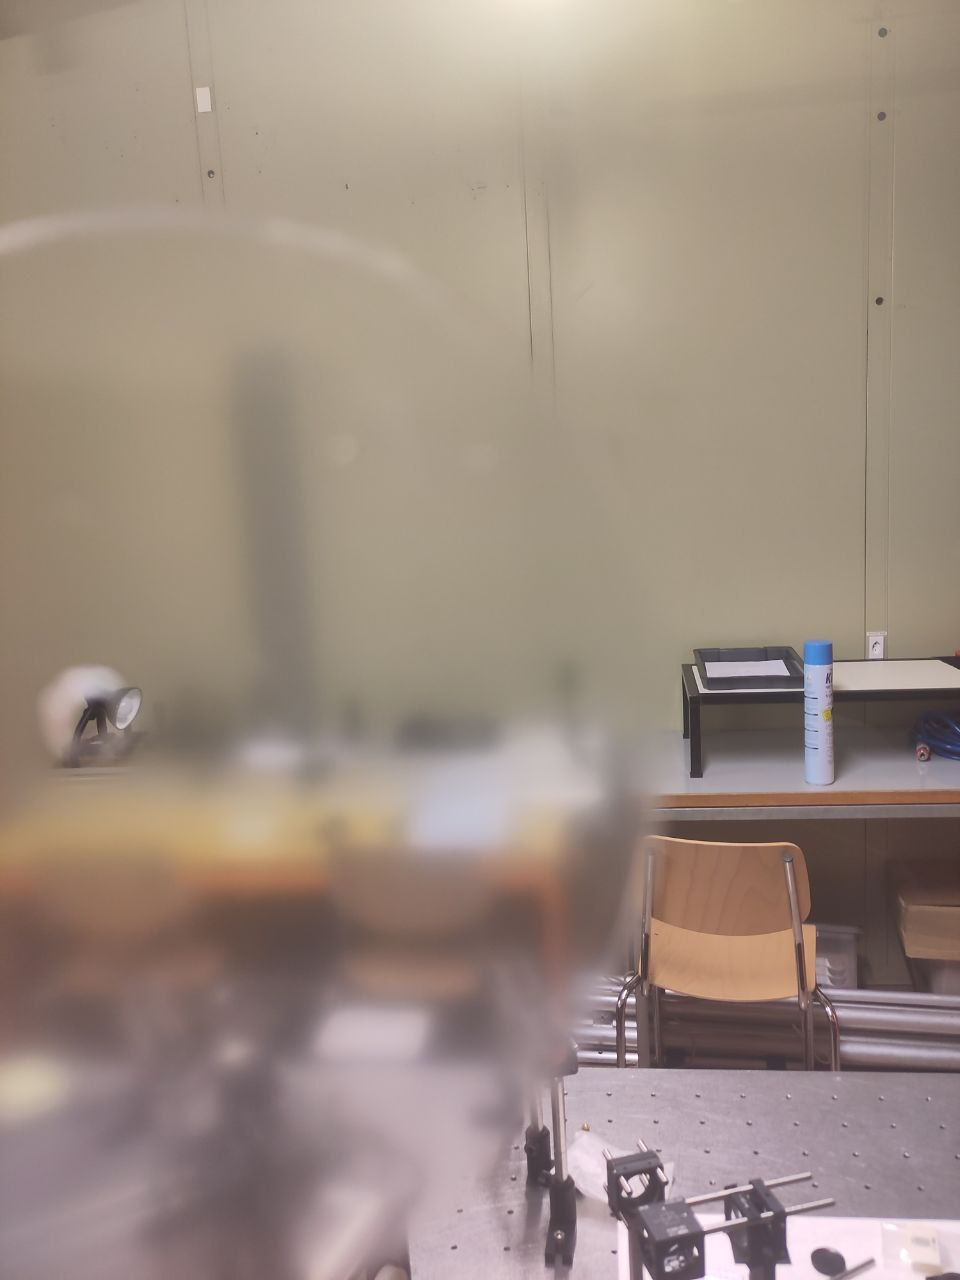
\includegraphics[width=1\linewidth]{assets/figures/mesures/60_sec_travers.jpeg}
        \caption{Vue au travers de l'écran de 60 secondes}
    \end{subfigure}
    \caption{Écran 60 secondes de côté et au-travers}
\end{figure}
Sur l'écran on peut observer des défaut, il y a eut des problèmes de buse lors de cette projection, il sera toutefois
intéressant de caractériser cet écran. Le nombre de prise de mesure est à chaque fois de 100 mesures.

\subsection{Script d'analyse des données}